\documentclass[10pt]{article}
\usepackage[letterpaper]{geometry}
\usepackage{listings}
\usepackage{color}
\usepackage{graphicx}
\definecolor{dkgreen}{rgb}{0,0.6,0}
\definecolor{gray}{rgb}{0.5,0.5,0.5}
\definecolor{mauve}{rgb}{0.58,0,0.82}

\lstset{frame=tb,
	language=C,
	aboveskip=3mm,
	belowskip=3mm,
	showstringspaces=false,
	columns=flexible,
	basicstyle={\small\ttfamily},
	numbers=none,
	numberstyle=\tiny\color{gray},
	keywordstyle=\color{blue},
	commentstyle=\color{dkgreen},
	stringstyle=\color{mauve},
	breaklines=true,
	breakatwhitespace=true,
	tabsize=3
}


\title{\textbf{Tarea: Calculadora con procesos}}
\author{Diego Ruiz Mora | 2202000335}
\date{9-Septiembre-2023}

\begin{document}
		
	\maketitle
	\section{Creación de procesos para cada operación}
	Para iniciar, será necesario crear los procesos que nos ayudarán a realizar las operaciones correspondientes de suma, resta, multiplicación y división. En los cuales el código es bastante sencillo, como podemos apreciar en los siguientes imágenes:
	
	\begin{figure}[h!]
		\centering
		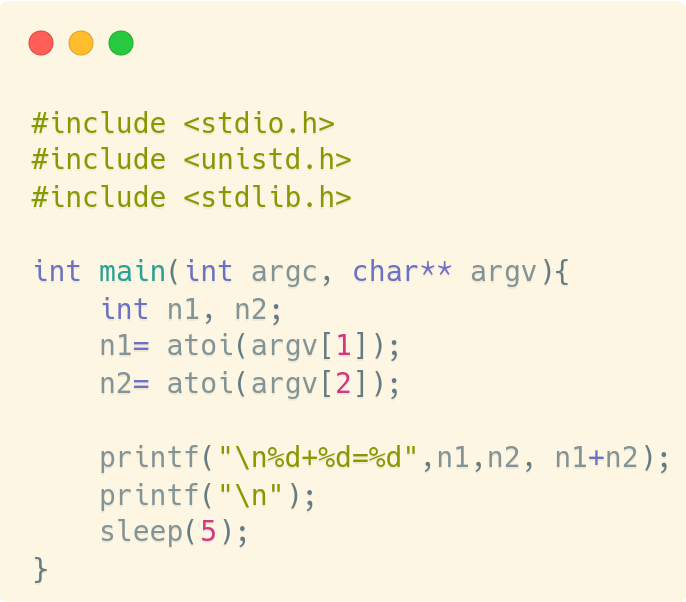
\includegraphics[width=0.5\linewidth]{suma.png}
		\caption{Código de suma.c}
		\label{fig:suma}
	\end{figure}
	
	Podemos notar de manera clara que en el código recibimos los parámetros, que en este caso tenemos el primero de ellos se refiere a la longitud del vector, que es el segundo parámetro que pasamos al 'main'. Este vector es de cadenas que termina con un '\textbf{NULL}, y al inicio tiene el comando con él que se invoca el programa, que en este caso sería \textbf{./suma}, en el medio tenemos algunos otros argumentos que se utilizarán en la ejecución de las instrucciones. 
	\\\\ 
	Esto se ve posteriormente en el código cuando de la tercera y cuarta posición del vector de argumentos obtenemos los números que vamos a sumar. Seguido, al efectuar la operación directamente lo imprimimos. Lo mismo sucederá en los siguientes casos, ya que las 4 primeras operaciones son sencillas de implementar. 
	\begin{figure}[h!]
		\centering
		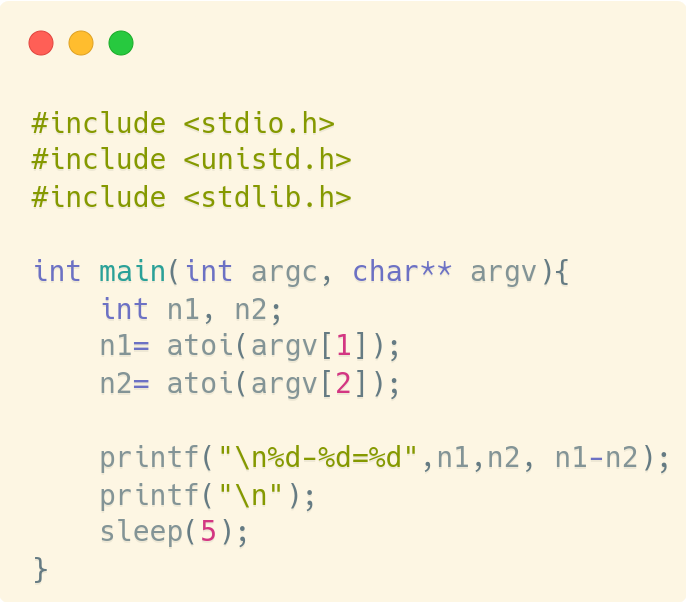
\includegraphics[width=0.5\linewidth]{resta.png}
		\caption{Código de resta.c}
		\label{fig:resta}
	\end{figure}
	\begin{figure}[h!]
		\centering
		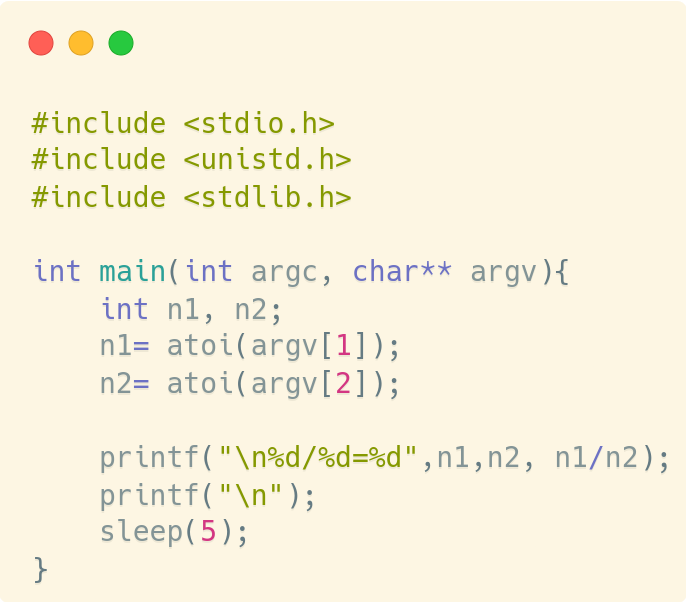
\includegraphics[width=0.5\linewidth]{division.png}
		\caption{Código de división.c}
		\label{fig:divsion}
	\end{figure}
	\begin{figure}[h!]
		\centering
		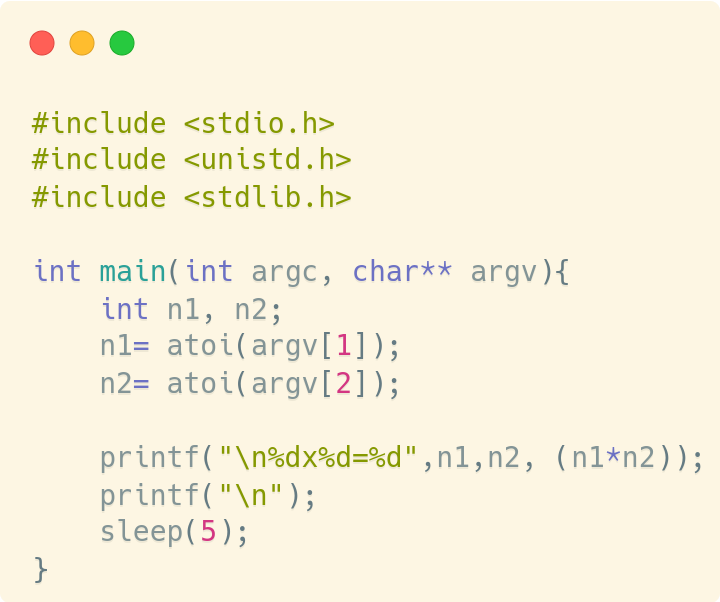
\includegraphics[width=0.5\linewidth]{multiplicacion.png}
		\caption{Código de multiplicación.c}
		\label{fig:multiplicacion}
	\end{figure}
	\\\\\\
	Como se puede apreciar cada uno de los códigos tienen una estructura parecida, solo difieren en la operación que realizan y en que como imprimen los datos, ya que tienen cada uno un operador distinto. Tal no es la situación al tener un procedimiento como los siguientes que son la permutación o la combinación, en tales caso tendremos que definir distintas funciones que nos permitan el calculo. 
	\begin{figure}[h!]
		\centering
		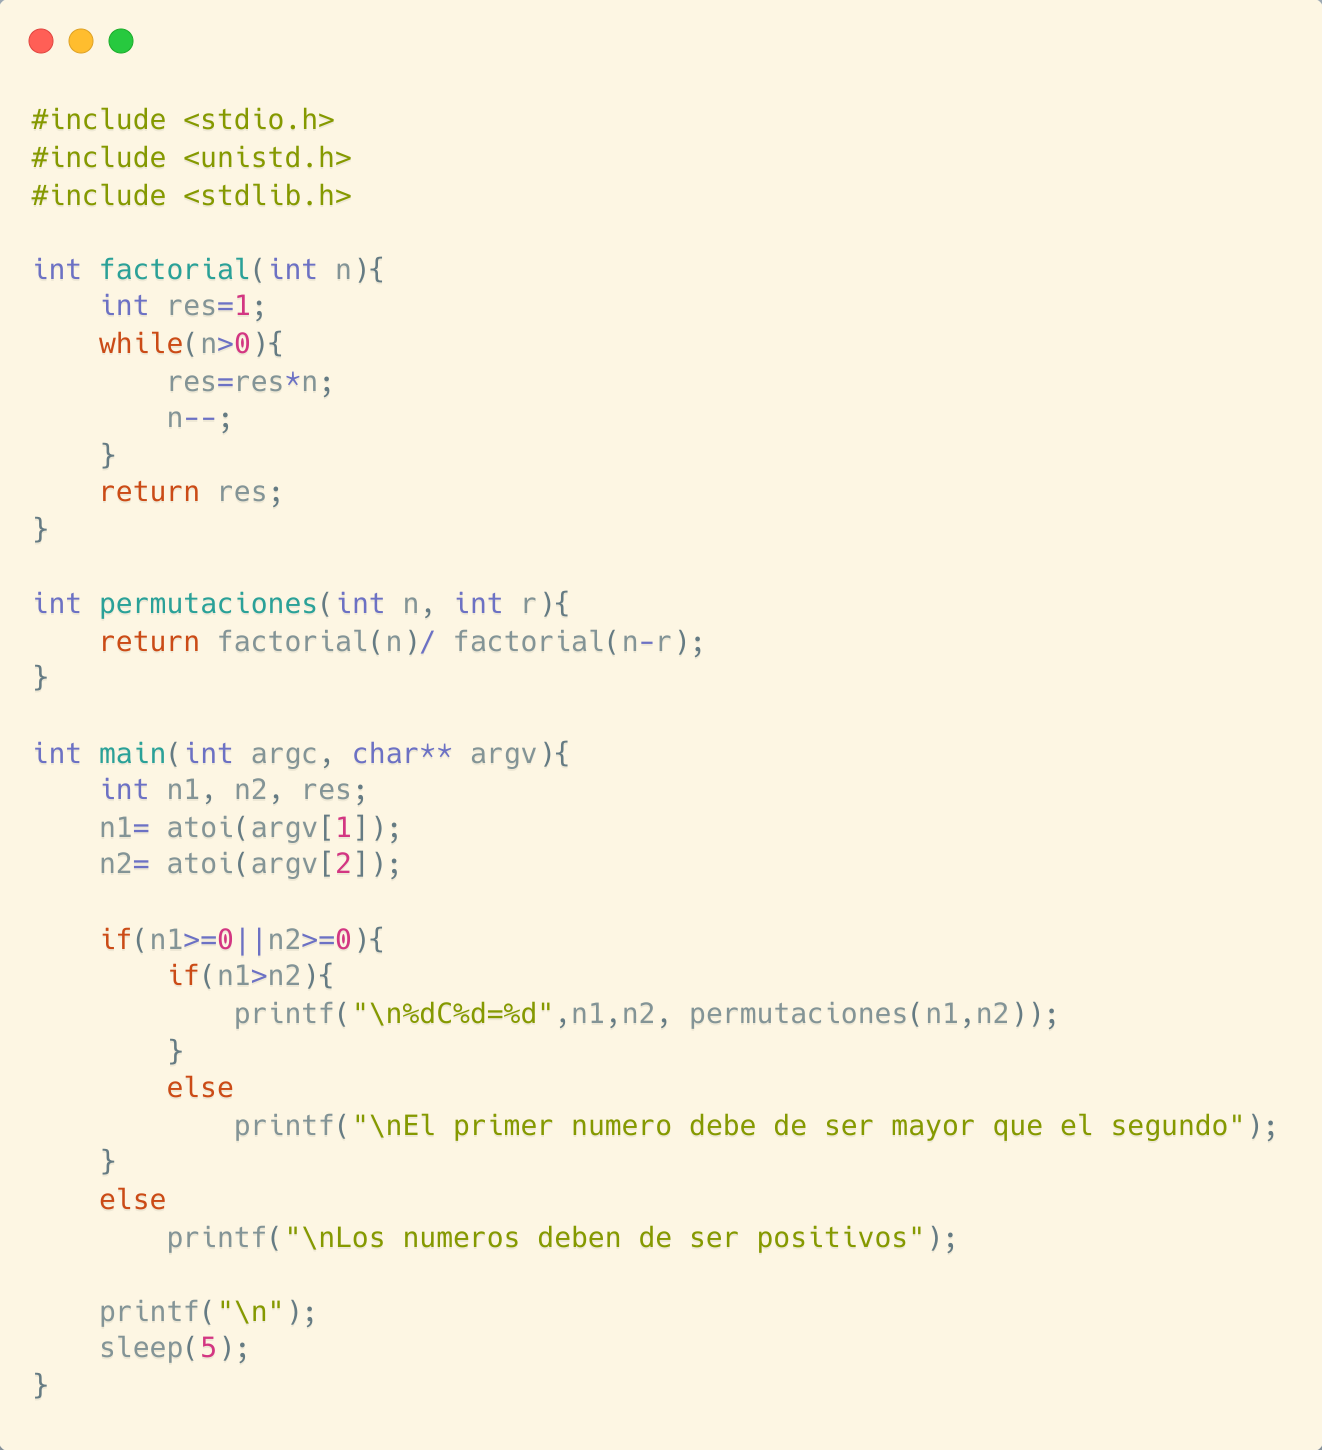
\includegraphics[width=0.7\linewidth]{permutaciones.png}
		\caption{Código de permutaciones.c}
		\label{fig:permutaciones}
	\end{figure}
	\newpage
	Primero tendremos que recordar que la fórmula para calcular el número de permutaciones y combinaciones:  
	\\\\
	\begin{equation}
		nPr=\frac{n!}{(n-r)!}
	\end{equation}
	\begin{equation}
		nCr=\frac{n!}{(n-r)!\ r!}
	\end{equation}
	\\\\
	Con el conocimiento de estas ecuaciones debemos de asumir que necesitamos una función que nos calcule el factorial y a su vez otra que nos calcule el numero de permutaciones para dos números dados, entendamos en ambas ecuaciones $(1)$ y $(2)$, a $n$ como el número de elementos tomados en rangos de $r$. Por tal razón, tendremos que mandar a llamar a la función factorial desde el cálculo de las permutaciones. 
	\\\\
	Por otro lado, en la función \textit{main} encontramos la función \textbf{atoi()} para hacer el \textit{casteo} de las cadenas encontradas dentro del vector de argumentos. Seguido tendremos que aplicar algunas condicionales para prevenir los posibles errores, como que se den elementos que sean igual a cero, o que tengamos que escoger grupos $r$ mayores que el numero de elementos $n$ (tal situación no existe en estos cálculos). 
	\\\\
	En cualquiera de los dos casos tendremos que advertir de lo que esta ocurriendo, esto se pudo haber solucionado desde la petición de los datos, pero se decidió hacer de esta forma debido a que las otras operaciones no tienen estas restricciones. Al final pondremos una pequeña detención del programa para que al momento de correrlo seamos capaces de ver que es lo que esta ocurriendo a nivel de procesos. 
	\newpage
	Será fácil deducir que en el caso de las combinaciones ocurre prácticamente lo mismo, con la ligera diferencia de la operación que realizaremos, en la \emph{figura \ref{fig:combinaciones}} tendrá el nombre de "combinaciones" asi como su repectiva ecuación $2$, pero fuera de eso se le da el mismo tratamiento a los datos y cuidamos exactamente los mismos aspectos relacionados con la naturaleza de los números (que no sean cero o menores, o que el segundo de ellos no sea mayor que el primero). 
	\begin{figure}[h!]
		\centering
		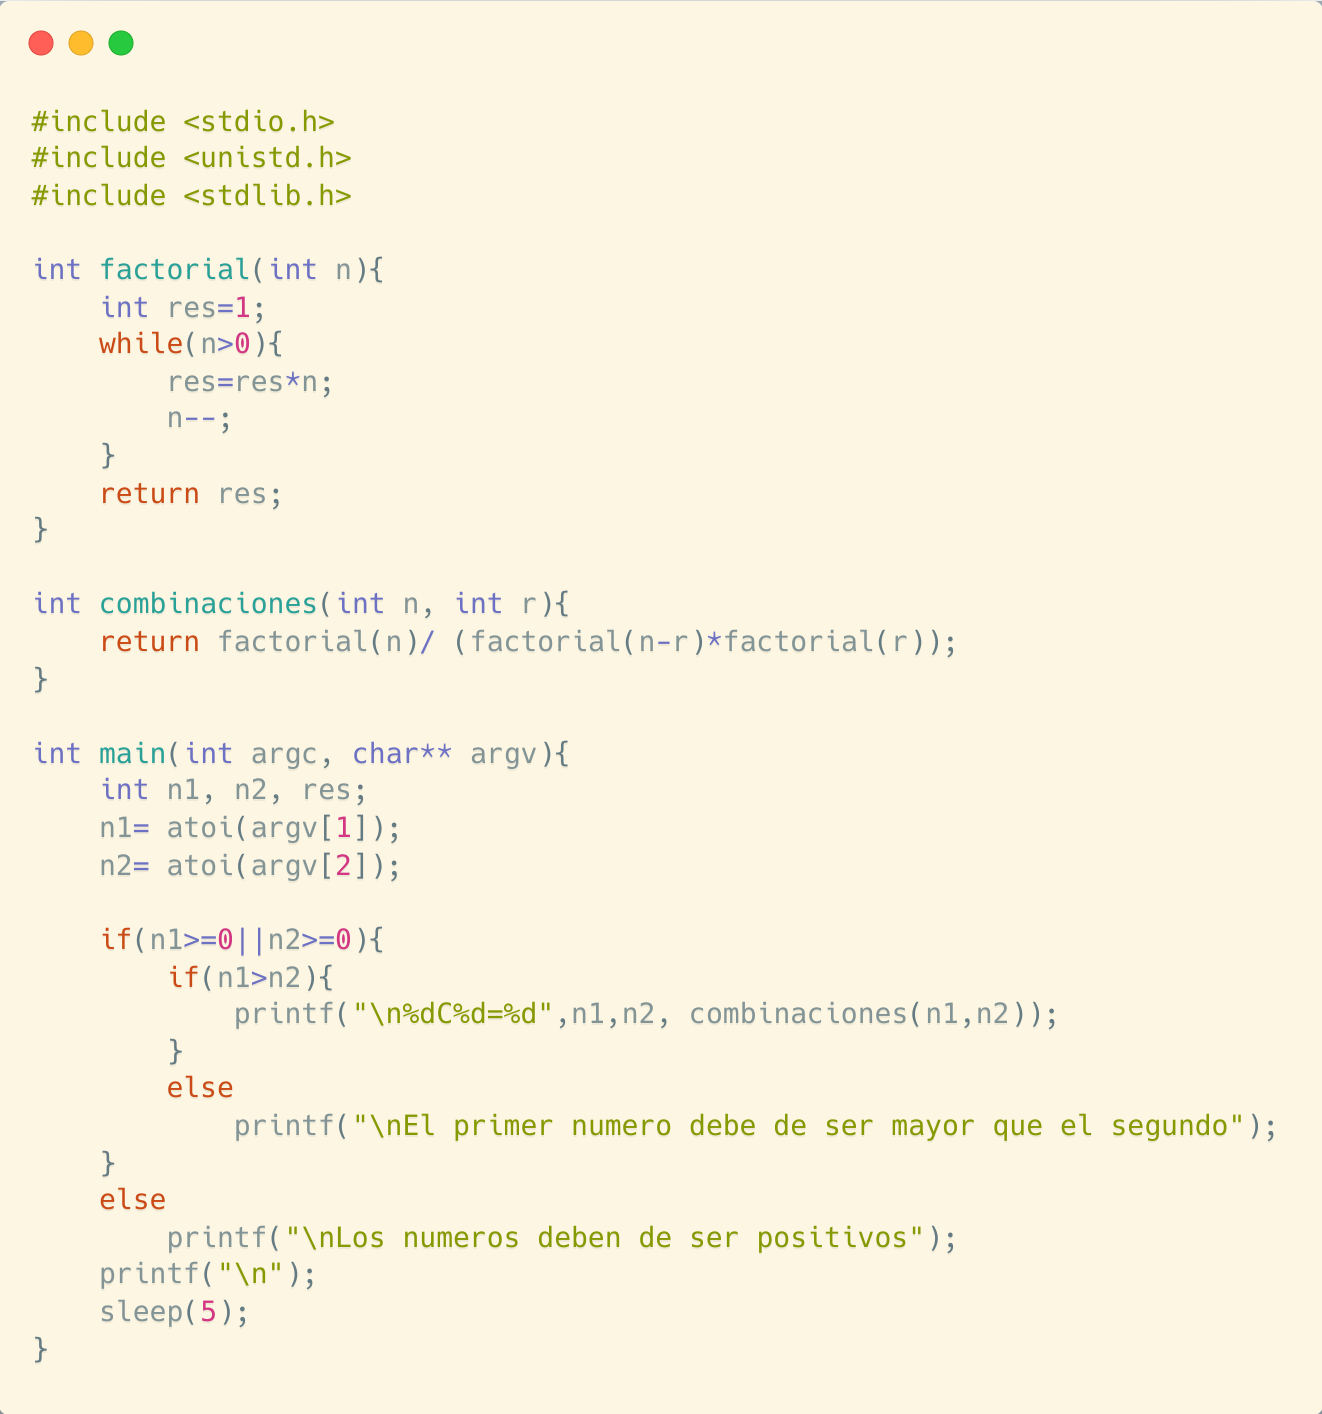
\includegraphics[width=0.7\linewidth]{combinaciones.png}
		\caption{Código de combinaciones.c}
		\label{fig:combinaciones}
	\end{figure}
	\newpage
	Quizá lo más interesante y el propósito principal de esta tarea recaiga en la parte relacionada con la función \emph{main}, donde encontraremos el uso de procesos más presente. Para ello quizá debamos de ver el código, primero que nada. 
	\\\\
	Este código lo encontramos en la \emph{figura \ref{fig:calculadora}}, al inicio se hace presente la petición de los datos, que en este caso y para ahorrarnos pasos decidimos hacerlo con \emph{cadenas}, ya que de una u otra forma los pasaremos con este tipo al vector de argumentos, lo cual se ve expresado en la asignación de los números a espacios particulares de la sección ($argv[1]=num1$). En seguida haremos la petición de la operación que queremos realizar, para ello utilizamos una estructura \emph{if-elseif-else}, pero sin antes realizar el clonado del proceso con la instrucción \textbf{fork()} que como vimos anteriormente nos creará un proceso hijo.
	\newpage
	A este proceso hijo le podremos pasar un cantidad de parámetros de tal manera que opere un código distinto, esto lo logramos con la instrucción \textbf{execve()}, la cual nos permite asignar el código distinto al hijo que acabamos de crear. De hecho, buscaremos asignar el código del proceso que es respectivo de la opción que se da un paso antes (suma, resta, multiplicación, división, permutaciones, combinaciones), dentro de cada una de las opciones asignaremos el identificador de los procesos, por ejemplo \emph{argv[0]="./suma"} para el caso de la suma. 
	\\\\
	\begin{figure}[h!]
		\centering
		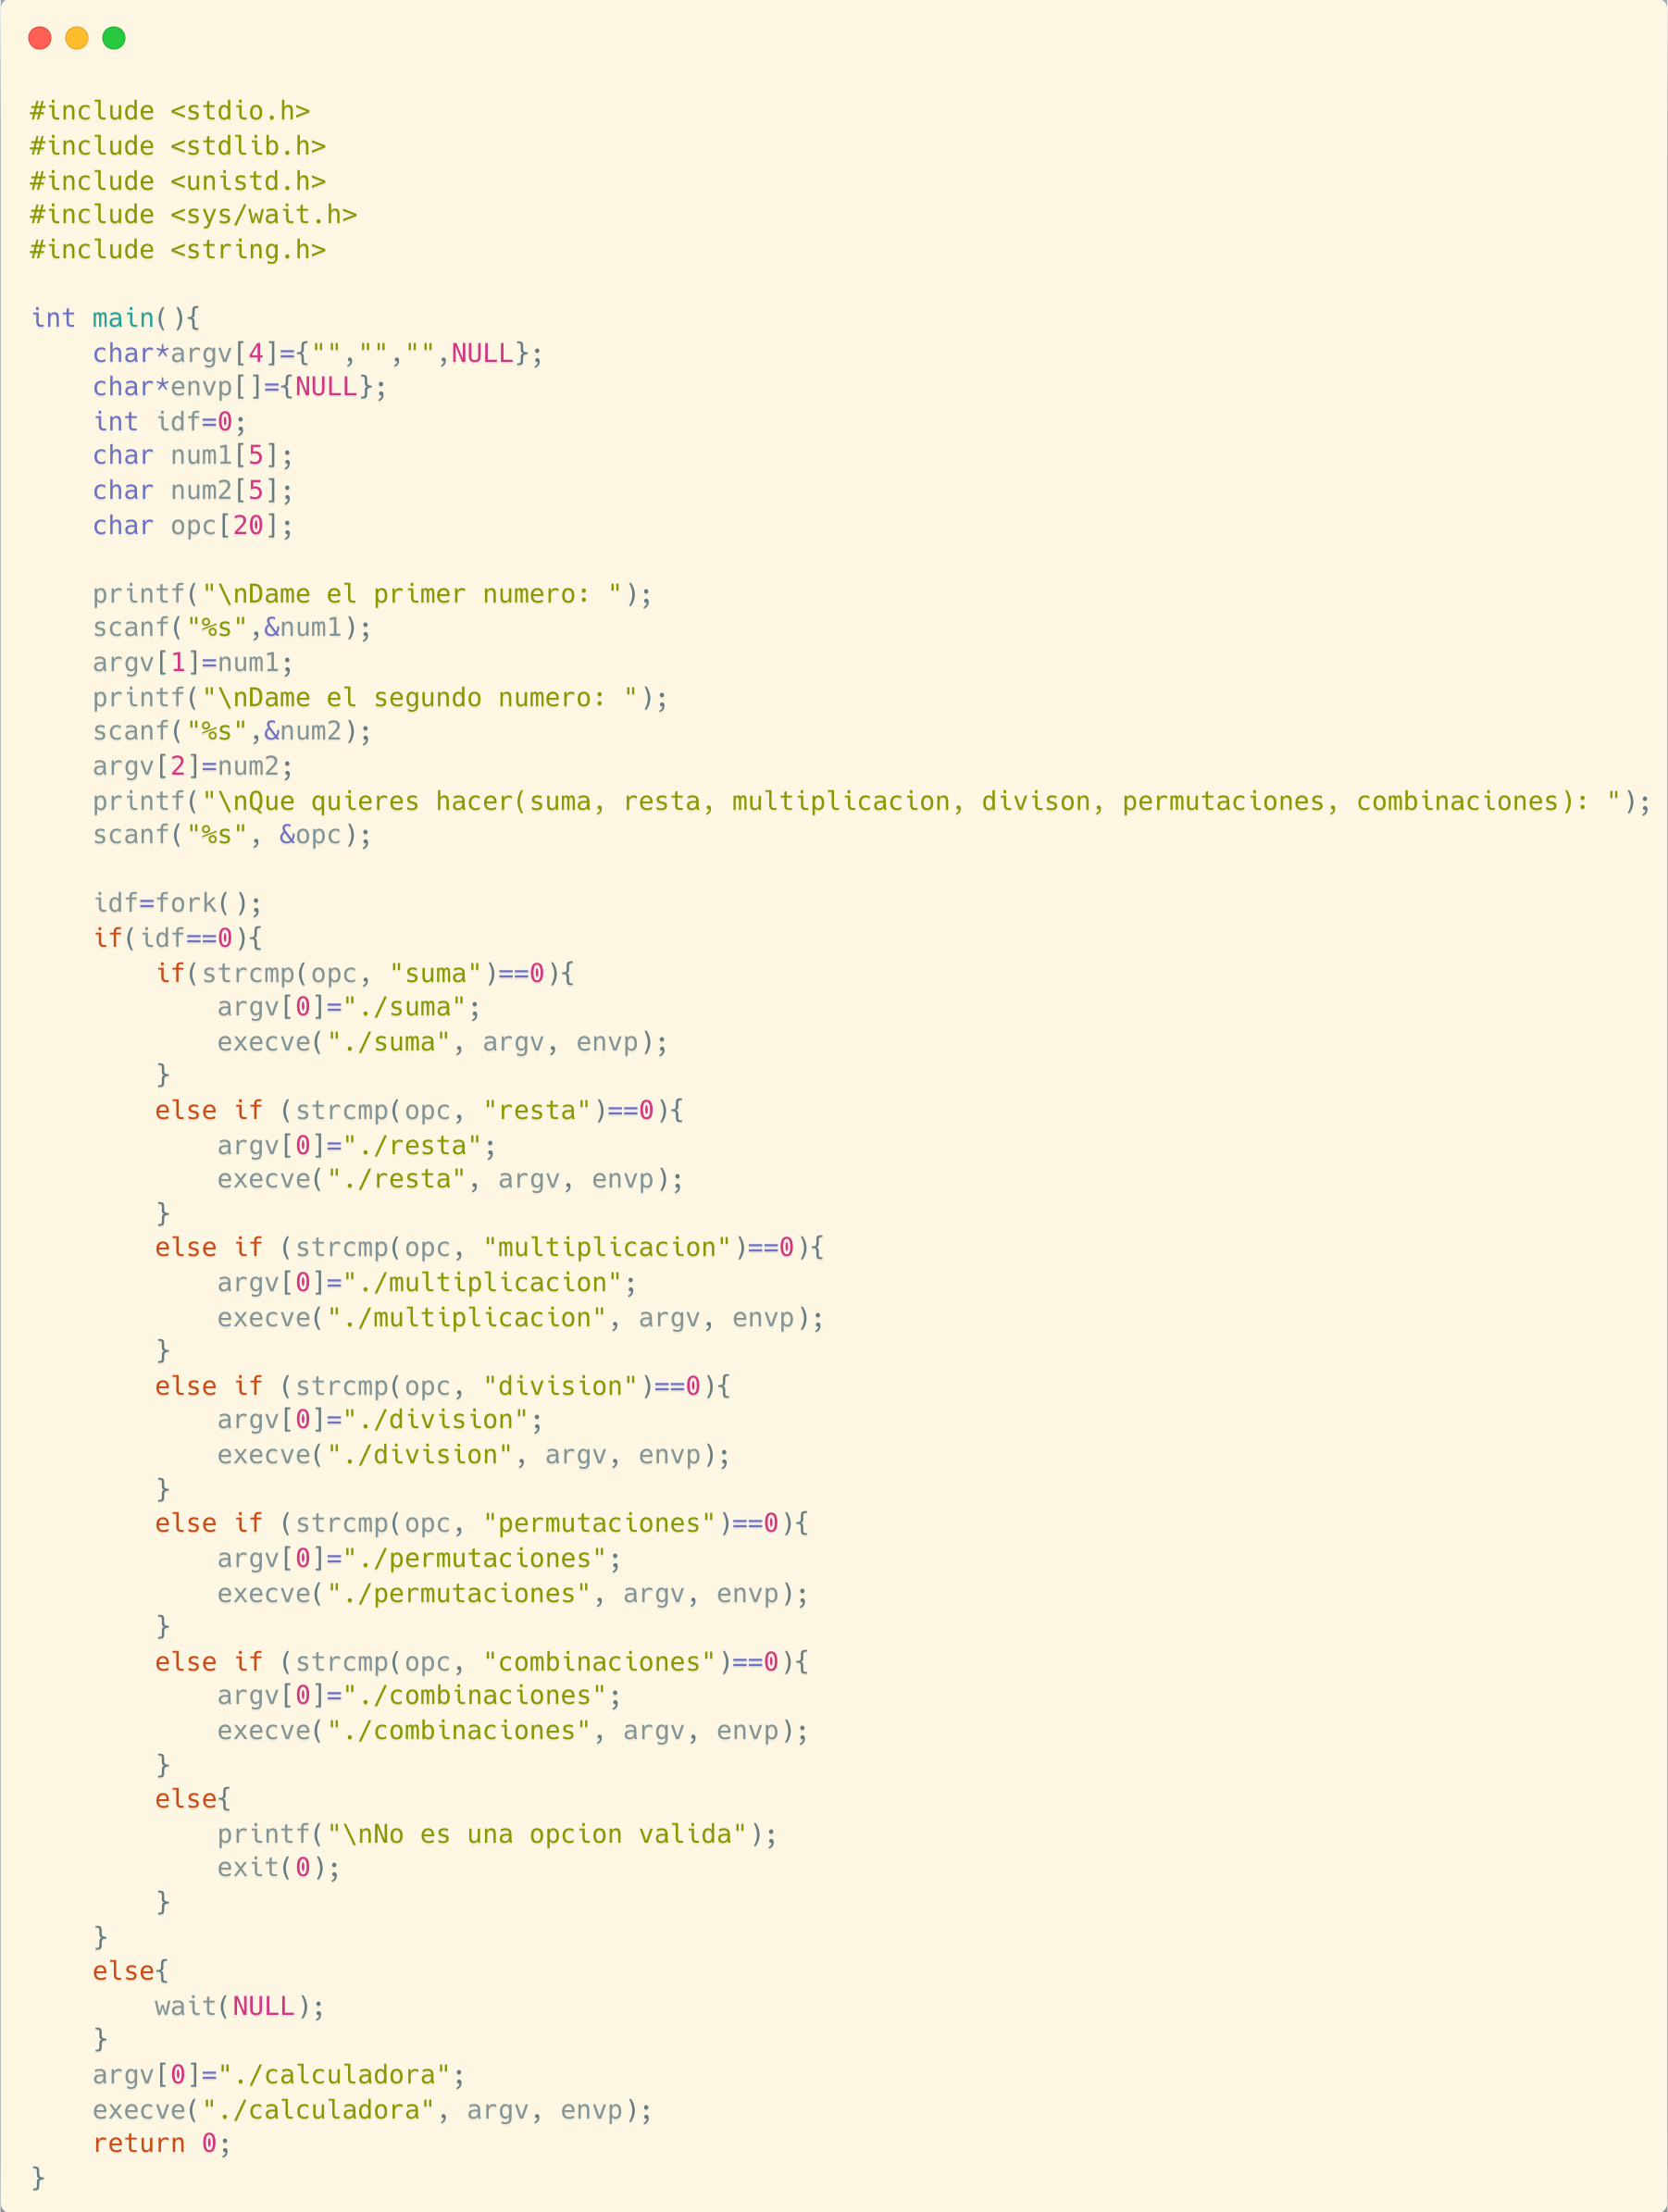
\includegraphics[width=0.7\linewidth]{calculadora.png}
		\caption{Código de calculadora.c}
		\label{fig:calculadora}
	\end{figure}
	\newpage
	Esto tiene suma importancia ya que la instrucción \textbf{execve()} tendremos como parámetros primero el nombre del proceso que mandaremos a llamar, luego el vector de argumentos (\textbf{argv}) y por un vector de apuntadores para las variables de estado, que denominamos \textbf{envp}, dentro del vector de argumentos encontramos lo siguiente: 
	\begin{enumerate}
		\item El procedimiento al que queremos mandar a llamar para copiar el código al hijo. 
		\item El primer número $n_1$ a operar. 
		\item El segundo número $n_2$ a operar. 
		\item NULL. Que funciona como un tipo de indicador para decir que el vector de argumentos ya termino. 
	\end{enumerate}
	Es importante notar que todas estas opciones se encuentran dentro de un \textbf{if} que nos hace modificar exclusivamente el código del proceso hijo (\textbf{idf==0}), en caso de no ocurrir esto simplemente hará un espera a que proceso padre se termine de ejecutar después de que el hijo termine su ejecución,  incluso podríamos omitir este \textbf{else} ya que lo realmente importante es discriminar la ejecución de estas instrucciones solamente al proceso hijo. 
	\\
	Así mismo en caso de querer ingresar una opción invalida para la operación a realizar se generará una advertencia de que tal opción no es valida. Además de que ejecutará la instrucción \textbf{exit(0)} que terminará el proceso actual, que en este caso será el proceso hijo. Y no se vayan acumulando todos los procesos al llegar al final. 
	\\\\
	Por último, pero yo creo que bastante importante, es la llamada al mismo proceso calculadora, para ello se modifica el vector de argumentos en su primera posición e incorporamos la instrucción \textbf{execve} mandando a llamar al mismo proceso, para así generar un menú que se repita para hacer muchas operaciones, en este caso no nos interesa cuales sean los otros argumentos, ya que verdaderamente no tenemos como tal el recibimiento de los argumentos para la función \emph{main} de este proceso. 
	\\\\
	En las siguientes imágenes veremos como es que opera, en este caso con el uso de la herramienta \emph{htop} para notar de manera clara cada uno de los procesos y los argumentos que recibe.
	\\
	En la \emph{figura \ref{fig:prueba1}}  podemos notar como en la petición de los datos aun seguimos dentro del proceso padre, después de que demos la operación y demos 'enter' debería de aparecer un nuevo proceso que tenga el nombre de la operación que se esta realizando, como en la \emph{figura \ref{fig:prueba2}}, donde se ve como el proceso se llama \textbf{"./suma"} y tiene como parámetros \emph{12} y \emph{13} que son los valores que se pasaron. 
	\\\\
	Luego de ello, al terminar la operación tenemos que este proceso \emph{suma} creado deja de aparecer y solamente aparece el procedimiento padre que es el producto de la ultima instrucción que manda a llamar al mismo proceso. Hay que denotar que el uso de esta instrucción sale de las instrucciones que ejecutan los hijos, por lo que solamente lo hará el padre, es como sobrescribir el programa. Cabe decir, que esta instrucción la pudimos incorporar en el \textbf{else} de la comparación \textbf{idf==0}.
	\begin{figure}[h!]
		\centering
		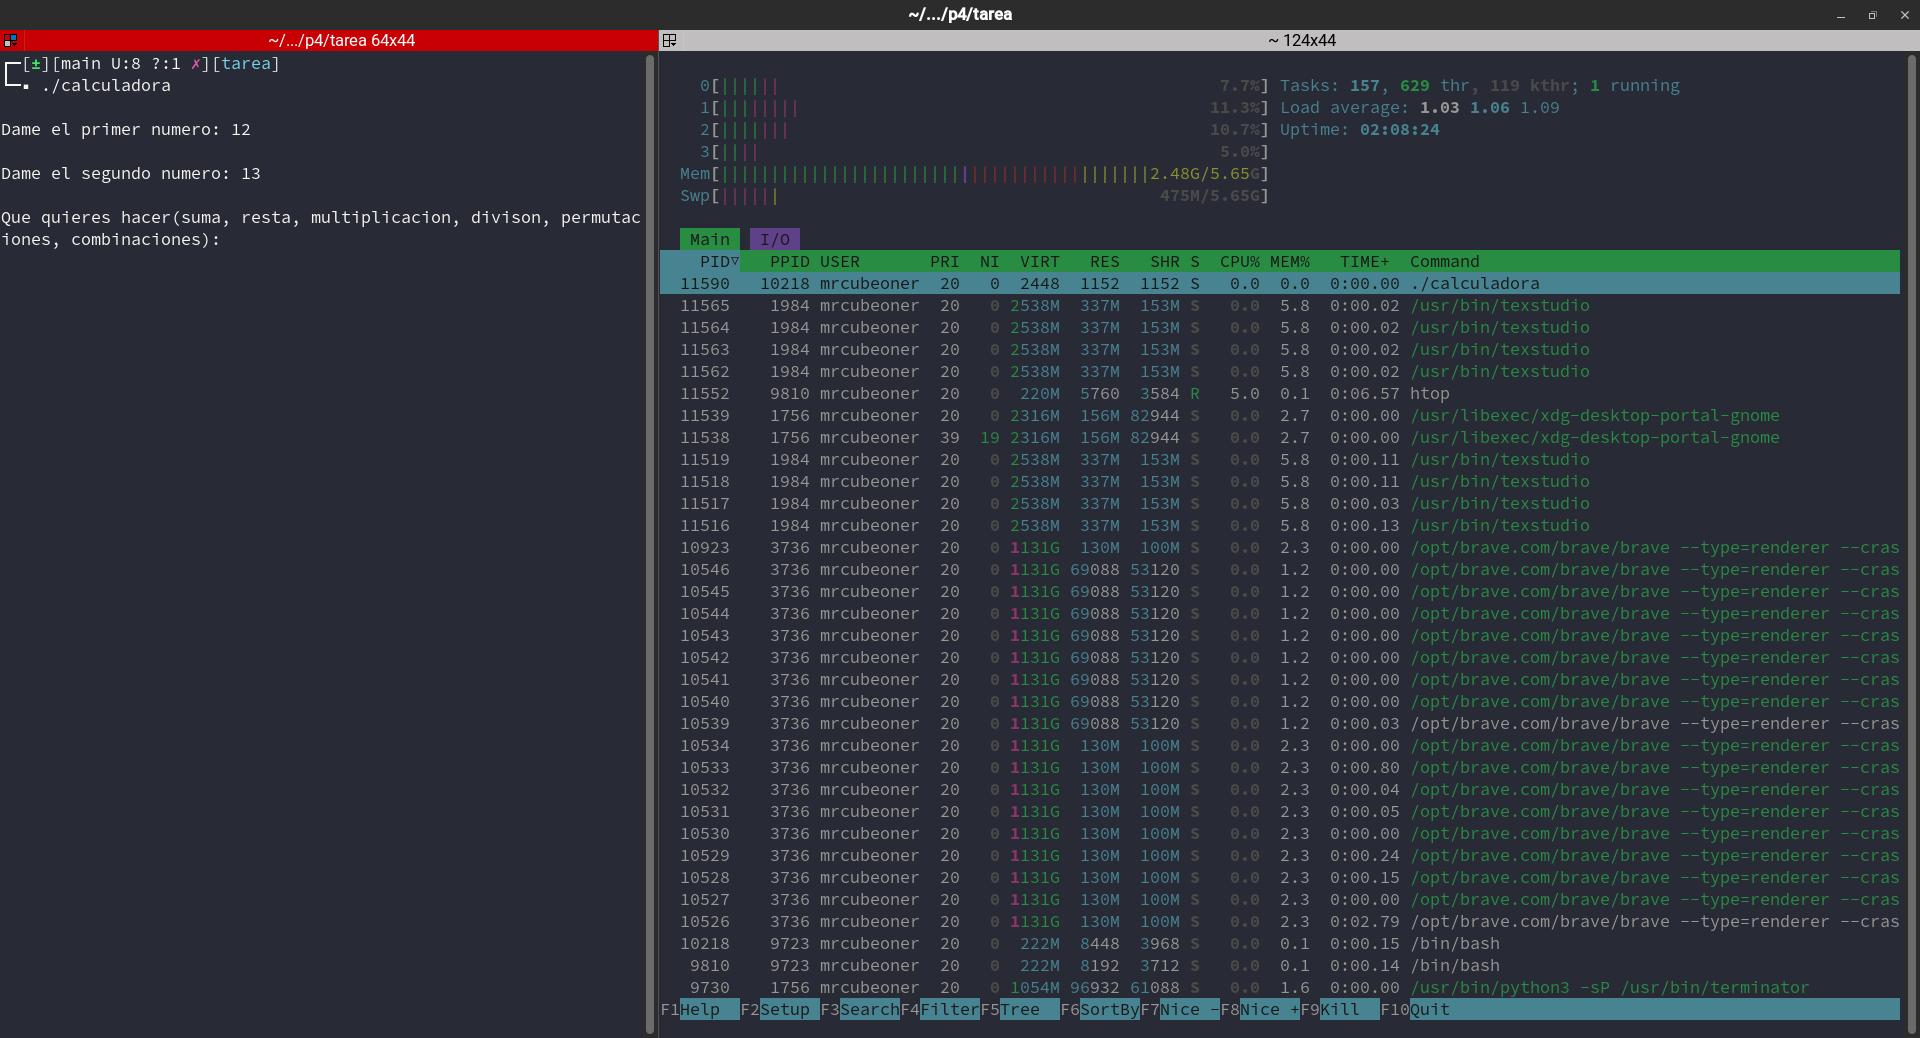
\includegraphics[width=1\linewidth]{prueba1}
		\caption{Prueba 1.1}
		\label{fig:prueba1}
	\end{figure}
	\begin{figure}[h!]
		\centering
		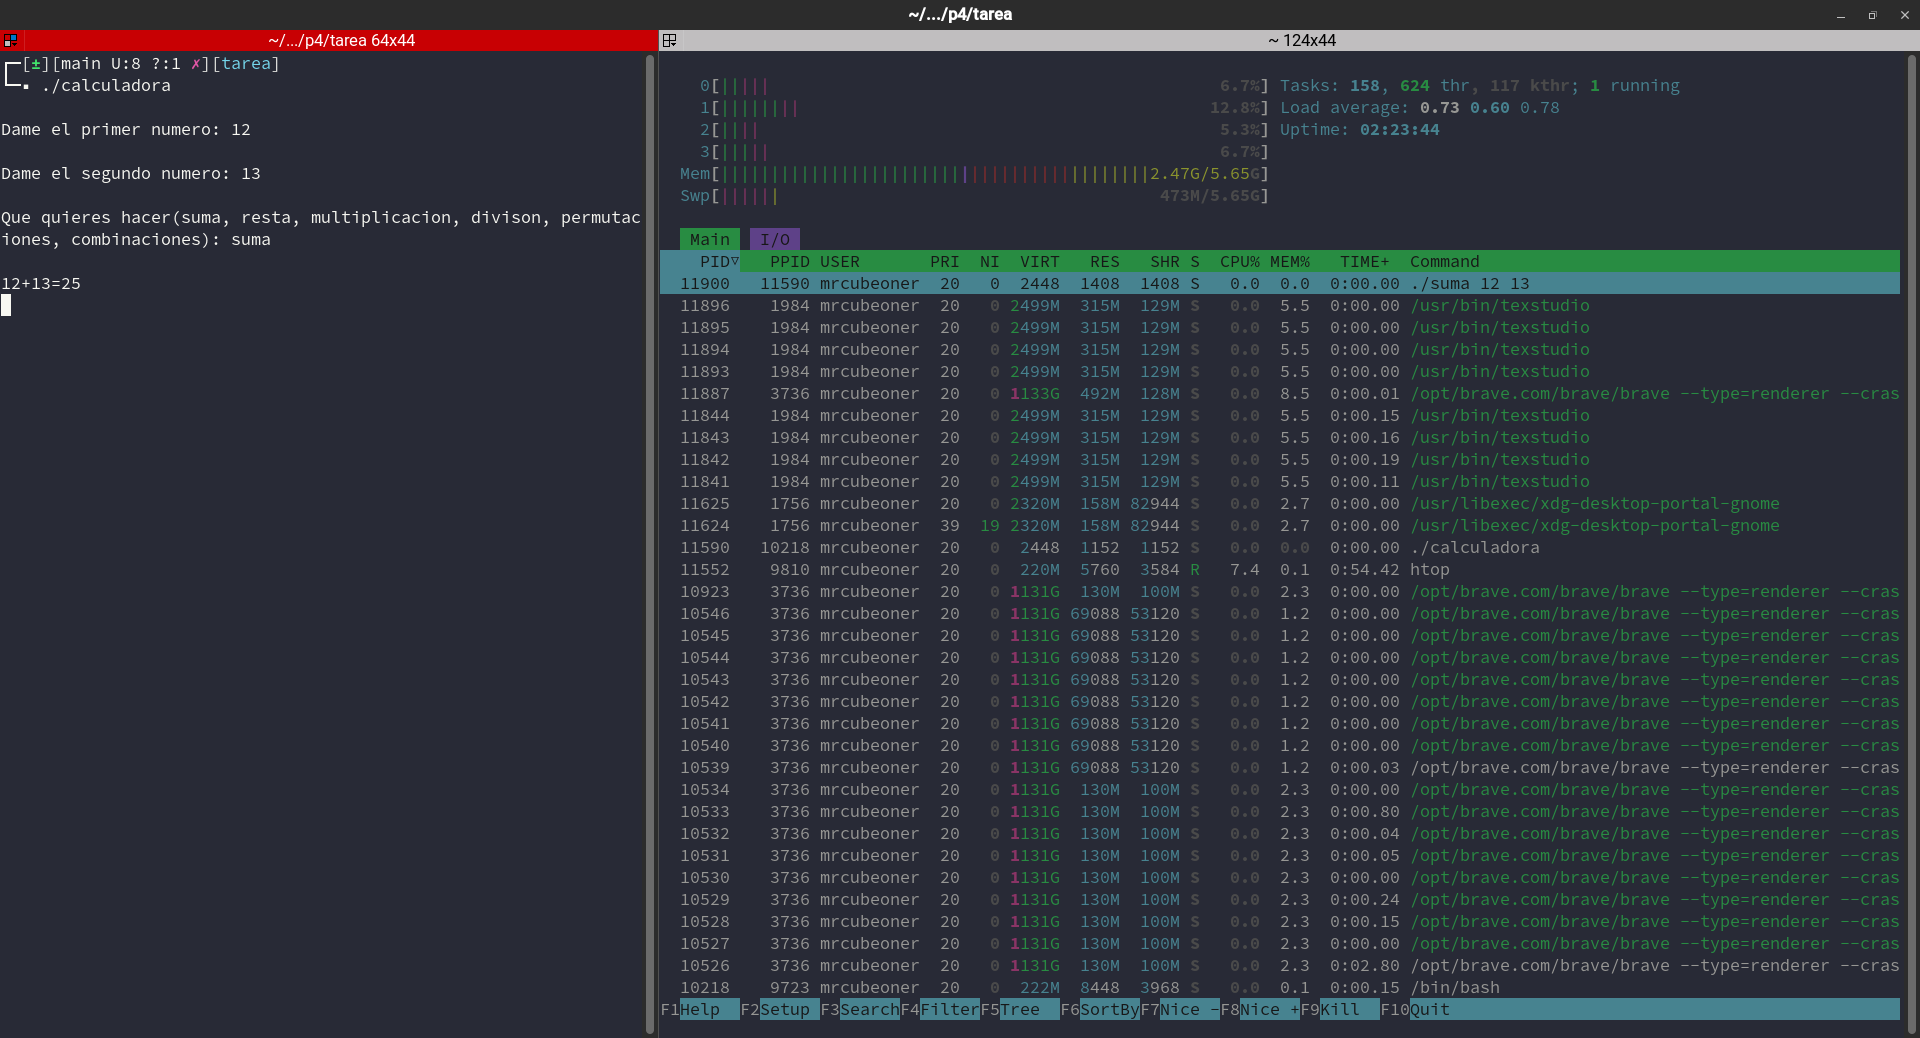
\includegraphics[width=1\linewidth]{prueba2}
		\caption{Prueba 1.2}
		\label{fig:prueba2}
	\end{figure}
	\begin{figure}[h!]
		\centering
		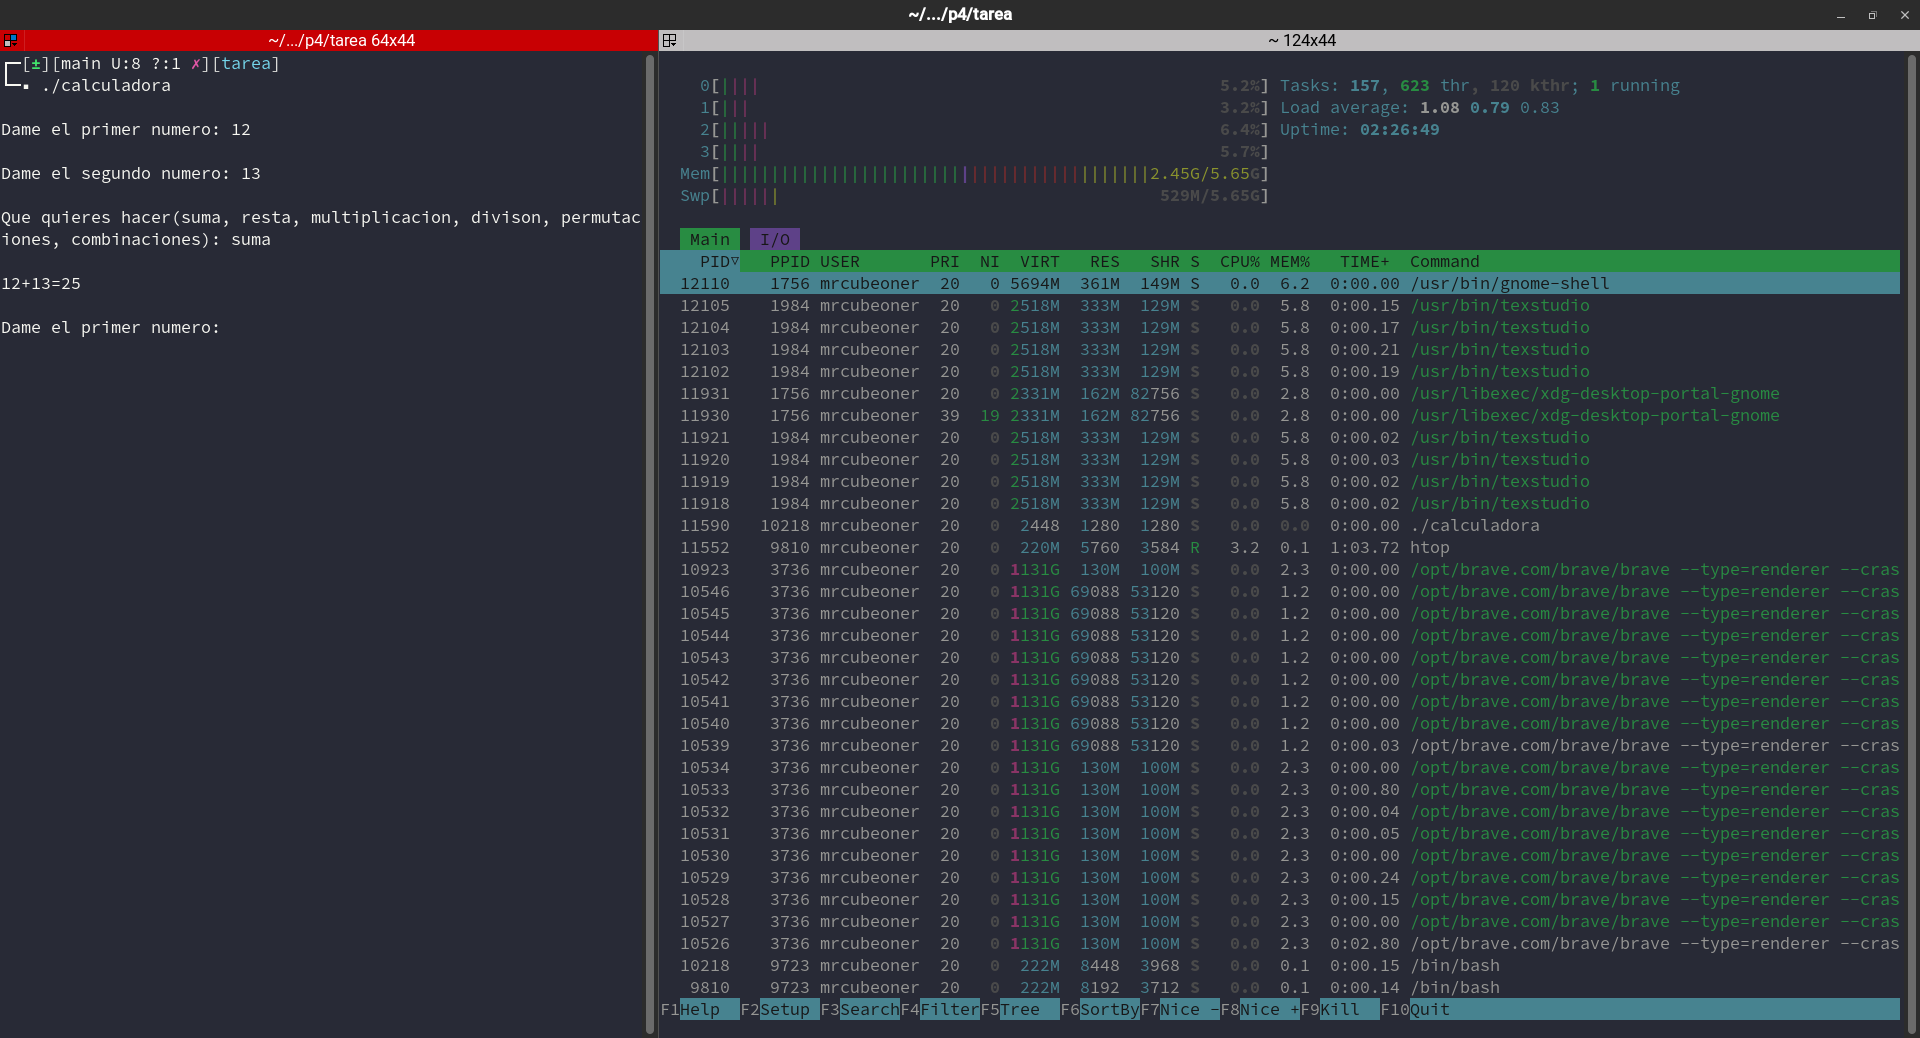
\includegraphics[width=1\linewidth]{prueba3}
		\caption{Prueba 1.3}
		\label{fig:prueba3}
	\end{figure}
	
	
\end{document}